\documentclass[11pt,a4paper,titlepage]{article}
\usepackage[left=2cm,text={17cm,24cm},top=3cm]{geometry}
\usepackage[T1]{fontenc}
\usepackage[czech]{babel}
\usepackage[utf8]{inputenc}
\usepackage{listings}

\usepackage{graphicx}

\usepackage{hyperref} % url

\bibliographystyle{czplain}

%uvozovky
\newcommand{\ceskeuvozovky}[1]{\quotedblbase#1\textquotedblleft}
\begin{document}

\begin{titlepage}
\begin{center}
    {\LARGE\textsc{Vysoké učení technické v~Brně}}\\
    \smallskip
    {\Large\textsc{Fakulta informačních technologií}}\\
    \bigskip
    \vspace{\stretch{0.382}}
    \LARGE{Modelování a simulace - projekt}\\
    \smallskip
    \Huge{Produkce řepky v ČR}\\
    \vspace{\stretch{0.618}}
\end{center}
    {\Large Petr Kapoun - xkapou04 \\ Erik Kelemen - xkelem01 \hfill \today }
\end{titlepage}

\tableofcontents
\newpage


\section{Úvod}
Našim cílem je simulovat růst řepky, při kterém se zameříme na co nejefektivnejší využití zemědělských strojů na sázení, postřik, rozmetání hnojiv, sklizeň a přepravu do skladu. Neklademe si však za cíl přesně určit výnos řepky, spíše určit percentuální ztráty, v důsledku infestace škůdci, nebo naopak navýšení úrody v důsledku poctivého hnojení. Simulace sleduje také použité zdroje jako náklady za pohonné látky, postřik a podobně. Pak už záleží jen na uživateli, či simulované navýšení úrody stojí za náklady spojené s jeho realizací.



\section{Postřiky}
Zvolili jsme kompletní řešení postřiků od fitmy BASF\footnote{BASF je německá agrochemická firma, která patří k 
největším na světě.\\https://www.agro.basf.cz/agroportal/cz/cs/startpage.html.}.
Pro určení přibližné ceny jednotlivých postřikových přípravků použijeme ceny existujícího eshopu obchod.agrokop.cz\footnote{AGROKOP CZ, a.s. Třebíč}.
\begin{figure}[ht!]
\centering
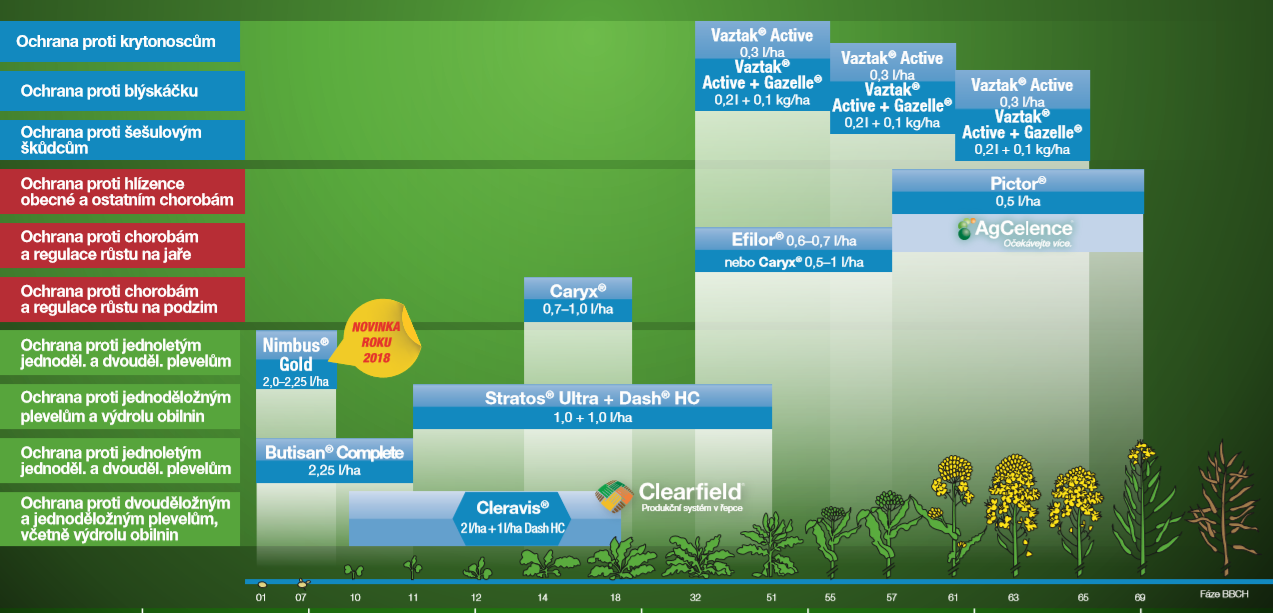
\includegraphics[width=170mm]{img/postriky}
\caption{Ochrana řepky proti škodlivým činitelům firmy BASF \label{basf_postriky}}
\end{figure}
Používané přípravky se dělí do několika skupin, to je důležité hlavně kvůli informaci o mísitelnosti jednotlivých přípravků.
\begin{itemize}
  \item Listová hnojiva.
  \item Fungicidy.
  \item Insekticidy.
  \item Herbicidy.
  \item Graminicidy.
\end{itemize}

\subsection{Ochrana proti krytonoscům, blýskáčku a šešulovým škůdcům}
Použitý přípravek se nazývá Vaztak Active\footnote{Vaztak je přípravek německého výrobce BASF: \\\url{\detokenize{
https://www.agro.basf.cz/agroportal/cz/cs/crop_protection/vyhled_v_n__p__pravk__podle_parametr_/product_details_24923.html
}}
\\\url{\detokenize{
https://www.agro.basf.cz/agroportal/cz/media/migrated/product_files/charakteristiky/CH_Vaztak_Active.pdf}}.}.
Je určený proti 
některým  druhům  žravého  a  savého  hmyzu,  jeho  larvám  a  vajíčkům.  Účinkuje  
jako dotykový a požerový jed.

\begin{itemize}
  \item Spotřeba 0,3l/ha. * 3 za každé období postřiku.
  \item Doporučené množství vody 200–600 l/ha (polní plodiny, zelenina), 200–1000 l/ha (prostorové plodiny) 
  \item Kategorie Insekticidy.
  \item Mísit lze se vším.
  \item Cena 815 bez DPH za litr.
\end{itemize}

\subsection{Ochrana proti hlízence obecné a ostatním chorobám}
Použitý přípravek se nazývá Pictor\footnote{Pictor je přípravek německého výrobce BASF: \\\url{\detokenize{
https://www.agro.basf.cz/agroportal/cz/cs/crop_protection/vyhled_v_n__p__pravk__podle_parametr_/product_details_1396.html
}}
\\\url{\detokenize{https://www.agro.basf.cz/agroportal/cz/media/migrated/information_material/brochures_products_1/brochures_products/2014/Pictor_Errata.pdf}}
.}.
\begin{itemize}
  \item Spotřeba 0,5l/ha.
  \item Doporučené množství vody 200-400l/ha.
  \item Kategorie Fungicidy.
  \item Mísit lze se vším.
  \item Cena 3280 bez DPH za litr.
  \item Hlízenka obecná může způsobit výnosové 
ztráty až 30 \%
\end{itemize}


\subsection{Ochrana proti chorobám a regulace růstu na jaře}
Použitý přípravek se nazývá Efilor\footnote{Efilor je přípravek německého výrobce BASF: \\\url{\detokenize{
https://www.agro.basf.cz/agroportal/cz/cs/crop_protection/vyhled_v_n__p__pravk__podle_parametr_/product_details_72192.html
}}.}.
Efilor zajišťuje ochranu proti houbovým chorobám.
\begin{itemize}
  \item Spotřeba 0,6l/ha.
  \item Doporučené množství vody 150-400l/ha.
  \item Kategorie Fungicidy.
  \item Mísit nelze pouze pýrohubné dávky u Graminicidů.
  \item Cena 1399 bez DPH za litr.
\end{itemize}

\subsection{Ochrana proti chorobám a regulace růstu na podzim}
Použitý přípravek se nazývá Caryx\footnote{Caryx je přípravek německého výrobce BASF: \\\url{\detokenize{
https://www.agro.basf.cz/agroportal/cz/cs/crop_protection/vyhled_v_n__p__pravk__podle_parametr_/product_details_1446.html
}}
\\\url{\detokenize{
https://www.agro.basf.cz/agroportal/cz/media/migrated/information_material/brochures_products_1/brochures_products/2014/Caryx_Errata.pdf
}}.}.
\begin{itemize}
  \item Spotřeba 0,75-1l/ha.
  \item Doporučené množství vody 150-400l/ha.
  \item Kategorie Fungicidy.
  \item Mísit nelze pouze pýrohubné dávky u Graminicidů.
  \item Cena 1009 bez DPH za litr.
\end{itemize}

\subsection{Ochrana proti jednoletým jednoděl. a dvouděl. plevelům}
První možný přípravek se nazývá Butisan Complete\footnote{Butisan Complete je přípravek německého výrobce BASF: \\\url{\detokenize{
https://www.agro.basf.cz/agroportal/cz/cs/crop_protection/vyhled_v_n__p__pravk__podle_parametr_/product_details_85632.html
}}.}.
\begin{itemize}
  \item Spotřeba 2-2,25l/ha.
  \item Doporučené množství vody 100-400l/ha.
  \item Kategorie Herbicidy.
  \item Mísit lze se vším.
  \item Cena 1016 bez DPH za litr.
\end{itemize}

\subsection{Ochrana proti jednoděložným plevelům a výdrolu obilnin}
Použitý přípravek se nazývá Stratos Ultra\footnote{Stratos Ultra je přípravek německého výrobce BASF: \\\url{\detokenize{
https://www.agro.basf.cz/agroportal/cz/cs/crop_protection/vyhled_v_n__p__pravk__podle_parametr_/product_details_1429.html
}}
\\\url{\detokenize{
https://www.agro.basf.cz/agroportal/cz/media/migrated/product_files/charakteristiky/CH_Stratos_Ultra.pdf
}}.}.
\begin{itemize}
  \item Spotřeba 1l/ha.
  \item Doporučené množství vody 200-300l/ha.
  \item Kategorie Herbicidy.
  \item Mísit nelze s listovým hnojivem Solubor.
\end{itemize}
Pomocný přípravek se nazývá Dash HC\footnote{Dash HC je přípravek německého výrobce BASF: \\\url{\detokenize{
https://www.agro.basf.cz/agroportal/cz/cs/crop_protection/vyhled_v_n__p__pravk__podle_parametr_/product_details_1441.html
}}.}.
\begin{itemize}
  \item Spotřeba 1l/ha.
  \item Doporučené množství vody 300l/ha.
\end{itemize}
Cena za 10l přípravku Stratos Ultra a 10l přípravku Dash HC je 6990 bez DPH.

\subsection{Ochrana proti dvouděložným a jednoděložnám plevelům, včetně výdrolu obilnin}
Použitý přípravek se nazývá Cleravis\footnote{Cleravis je přípravek německého výrobce BASF: \\\url{\detokenize{
https://www.agro.basf.cz/agroportal/cz/cs/crop_protection/vyhled_v_n__p__pravk__podle_parametr_/product_details_55941.html
}}
\\\url{\detokenize{
https://www.agro.basf.cz/agroportal/cz/media/migrated/product_files/charakteristiky/CH_Cleravis.pdf
}}.}.
Slouží k hubení jednoletých dvouděložných a jednoděložných plevelů.
\begin{itemize}
  \item Spotřeba 2l/ha.
  \item Doporučené množství vody 300-400l.
  \item Kategorie Herbicidy.
  \item Mísit nelze s Graminicidy.
\end{itemize}
Pomocný přípravek se nazývá Dash HC.
\begin{itemize}
  \item Spotřeba 1l/ha.
  \item Doporučené množství vody 300l/ha.
\end{itemize}
Cena za 10l přípravku Cleravis a 5l přípravku Dash HC je 11699 bez DPH.




\section{Hnojiva}
Zvolili jsme kompletní řešení postřiků od fitmy Timac AGRO\footnote{BASF je německá agrochemická firma, která patří k 
největším na světě.\\https://www.agro.basf.cz/agroportal/cz/cs/startpage.html.}.
\footnote{TIMAC AGRO je průmyslovou společností specializující se na pěstování půdy, výživu rostlin a zvířat.\\\url{\detokenize{
https://www.cz.timacagro.com/rostlinna-vyroba/plodinova-doporuceni/repka-olejka.htmll
}}.}.
Pro určení přibližné ceny jednotlivých postřikových přípravků použijeme ceny existujícího polského eshopu https://www.kupnawozy.pl a také
rakouského espohu https://www.samen-schwarzenberger.at. Z obrázku je patrné, že je možné si vybrat z některých produkrů, tedy není nutné použít všechny.
Proto jsme z nich vybrali jen některé. Informace o konkrétních hnojivech jsme vyčetli z oficiálních etiket produktů,
 které je možné nalézt na stránce eagri.cz
\footnote{Vyhledavač:\\\url{\detokenize{
http://eagri.cz/public/app/rhpub/hnojivaVerejnostQF.do
}}. Příklad etikety:\\\url{\detokenize{
http://eagri.cz/public/app/rhpub/etikety/etiketa_36439.pdf?id=36439
}}.}.
\begin{figure}[ht!]
\centering
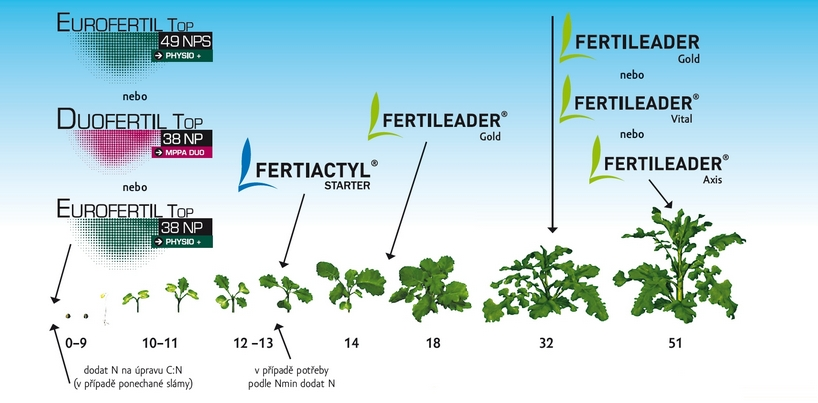
\includegraphics[width=170mm]{img/hnojiva}
\caption{Systém výživy a hnojení řepky ozimé firmy Timac AGRO \label{timac_hnojiva}}
\end{figure}

\subsection{Eurofertil Top 49 NPS}
Obsah látek: (NP 3/22; 24 SO3; 0,15 B; Mescal 975 (29 CaO); Physio+).
\begin{itemize}
  \item Spotřeba 150-250kg/ha.
  \item Cena 2425,0 PLN/t.
\end{itemize}

\subsection{Fertiactyl Starter}
Obsah látek: (13 \% N; 5 \% P2O5; 8 \% K2O; FERTIACTYL® komplex).
\begin{itemize}
  \item Spotřeba kg/ha.
  \item Spotřeba 3l/ha.
  \item Doporučené množství vody 150-500l/ha.
  \item Cena 62,4 PLN/l.
\end{itemize}

\subsection{Fertileader Gold}
Obsah látek: (5,7\%B + 0,35\%Mo + Seactiv).
\begin{itemize}
  \item Spotřeba 3l/ha.
  \item Doporučené množství vody 150-500l/ha.
  \item Cena 16,52 EUR/l.
\end{itemize}

\subsection{Fertileader Vital}
Obsah látek: (9\%N + 5\%P2O5 + 4\%K2O + 0,1\%Mn + 0,05\%B + 0,02\%Cu + 0,02\%Fe + 0,05\%Zn + 0,01\%Mo + Seactiv).
\begin{itemize}
  \item Spotřeba 4l/ha.
  \item Doporučené množství vody 150-500l/ha.
  \item Cena 15,99 EUR/l.
\end{itemize}



\section{Zemědělské stroje}

\subsection{Traktor a jeho závěsná zařízení}
Výhodou traktoru je jeho univerzálnost. Zvolili jsme traktor John Deere 6210R\footnote{Test traktoru John Deere 6210R: \\\url{\detokenize{
https://www.fwi.co.uk/machinery/mid-range-tractor-test-john-deere-6210r
}},
\\\url{\detokenize{
http://www.danhel.cz/fotogalerie/predvadeci-john-deere-6210r-s-directdrive.html
}}.}.
\begin{itemize}
  \item Spotřeba 37,1 litrů/h.
  \item Dopravní rychlost 13,8-42 km/h.
\end{itemize}

\subsubsection{Secí stroj}
Zvolili jsme secí stroj AMAZONE CAYENA, který si sám kypří půdu\footnote{Technické údaje o stroji AMAZONE CAYENA: \\\url{\detokenize{
https://www.zavesnatechnika.cz/seci-stroj-cayena
}}.}.
\begin{itemize}
  \item Pracovní rychlost 8-15 km/h.
  \item Pracovní záběr 6 m.
\end{itemize}

\subsubsection{Postřikový stroj}
Zvolili jsme nesené postřikovače AMAZONE UF s čelní nádrží FT\footnote{Technické údaje o stroji AMAZONE UF: \\\url{\detokenize{
https://www.zavesnatechnika.cz/obrazky-soubory/uf-a958a.pdf?redir
}}.}.
\begin{itemize}
  \item Pracovní rychlost 10 km/h.
  \item Pracovní záběr 12-30 m.
\end{itemize}

\subsubsection{Rozmetadlo minerálních hnojiv}
Zvolili jsme stroj AMAZONE ZA-M Ultra Profis Hydro\footnote{Technické údaje o stroji AMAZONE ZA-M: \\\url{\detokenize{
https://www.zavesnatechnika.cz/obrazky-soubory/prospekt_amazone_zam-55bc0.pdf?redir
}}.}.
\begin{itemize}
  \item Pracovní rychlost 12 km/h.
  \item Pracovní šířka 30 m.
  \item Pracovní rychlost 27 ha/h.
\end{itemize}

\subsubsection{Rozmetadlo minerálních hnojiv}
Zvolili jsme návěs T730/3\footnote{Technické údaje - NÁVĚS, 12T, T730/3: \\\url{\detokenize{
http://www.agrotechnika.cz/zemedelska-technika/navesy-12t-t730-3/
}}.}  s nosností 12t.
\begin{itemize}
  \item Objem 15,3 $m^3$.
\end{itemize}

\subsection{Sklízecí mlátička}
Zvolili jsme sklízecí mlátičku New Holland CR10.90\footnote{Technické údaje o sklízecí mlátičce CR10.90: \\\url{\detokenize{
https://www.eagrotec.cz/potvrzeno-zapisem-do-guinessovy-knihy-rekordu-sklizeci-mlaticka-cr10.90-je-nejvykonnejsi-mlatickou-na-svete
}}.}. Mlátička má i zásobník, do něj lze ukládat zrna v dobu sklizně. Odpad zůstává na poli.
Traktor zatím jezdí mezi mlátičkou a skladem, mlátička za jízdy přesypává svůj obsah na vůz za traktorem.
\begin{itemize}
  \item Spotřeba 11,14 litrů/ha.
  \item Rychlost 5,9 km/h.
  \item Rychlost sklizně 10,03 ha/h.
  \item Šířka žacího ústrojí: 6,10-12,5 m.
  \item Objem zásobníku zrna 14500 l.
  \item Rychlost vyprázdnění 142 l/m.
\end{itemize}

\section{Sledované statistiky}
\subsection{Úspešnost prací}
Nejdůležitější statistiky jsou právě statistiky úspešnosti, protože definují přibližné procento prací, které se vykonaly ze všech naplánovaných. Kolik procent hektarú orné půdy jsme stihli vysázet předtím než skončilo sázecí období nebo kolik procent hektarů řepky se stihlo postříkat/pohnojit před vypršením období na postřik/hnojení.
\subsubsection{Úspešnost sázení řepky}
Tato statistika závisí primárně na počtu hektarů orné půdy, času na sázení a počtu sázecích strojů. Když bude z této statistiky vycházet bezproblémové vysázení všech hektarů, indikuje to uživateli, že by mohl nakoupit víc orné půdy, zkrátit čas na sázení nebo prodat nějaký sázecí stroj.
\subsubsection{Úspešnost postřiků}
Tato statistika závisí na počtu hektarů řepky a postřikovačů. Tato statistika se eviduje pro každý postřik jednotlivě i společně pro všechny. Statistiky jsou časově závislé, v době kdy bude probíhat více postřiků najednou budou výsledky horší, protože budou postřikovače více vytížené. Další závislotí je, jestli se jedná o postřik selektivní nebo preventivní. Selektivní postřiky nemusí postřikovat celé pole, ale jenom nakažené časti pole. Ochranné postřiky budou aplikovány na celé pole. Uživatel může z těchto statistik zjistit období největšího vytížení postřikovačů a na tato období se podle toho adekvátně připravit pronajmutím dalších strojů nebo navýšením pracovních hodin.
\subsubsection{Úspešnost hnojení}
Tato statistika závisí na počtu hektarů řepky a rozmetadel minerálních hnojiv. Tato statistika se eviduje pro každé hnojivo jednotlivě i společně pro všechny. Časová závislost je stejná jako u postřiků. Znovu je statistika určena pro definování nejkritičtějších období, na které by se pak mohl uživatel(vlastník pole) připravit.
\subsubsection{Úspešnost sklizně}
Tato statistika závisí na počtu hektarů řepky a sklízecích strojů. Pro jakéhokoliv zemědělce je určitě jakákoliv jiná než stoprocentní sklizeň pole nepřípustná. Proto by si měl díky simulaci včas uvědomit, zdali mu daný počet strojů bude stačit.
\subsection{Voda}
Při simulaci se sleduje statistika použití vody. Jde o vodu použitou při postřicích. Její hodnota se nijak nepřevádí na cenové vyhodnocení, i když bychom mohli uvažovat cenu užitkové vody v českých korunách, není bežná praxe, aby si zemědělci vodu kupovali.

\subsection{Pohonné látky}
Při simulaci se sleduje statistika použití pohonných látek zemědělskými stroji. Tato statistika se pak odráží také v cenových nákladech, kde bude vyhodnocena pomocí kurzu jednoho litru pohonné látky na české koruny.

\subsection{Výnos}
Simulace vyhodnotí také předpokládaný výnos řepky v tunách. Ten se bude odvíjet od průměrného výnosu za hektár (Tuto hodnotu získáme třeba zde \detokenize{https://www.vynosy-plodin.cz/2018-okresy-repka-ozima/}). Do tohoto výnosu zasáhnou postřiky a hnojiva, které tento výnos ovlivní.

\pagebreak
\section{Implementace}
Diskrétní simulaci řídí algoritmus "next event". Čas simulace je vždy jeden rok, protože léta se vzájemne neovplyvňují a tudíž by sme pořád získavali približne stejné informace z každého roku.
Pro jednoduché ovlivňování parametrů simulace byl implementován syntaktický analyzátor jednoduchého konfiguračního(config) souboru.

\subsection{Petriho sítě}
Modelovali jsme diskrétní systém pomocí hierarchické petriho sítě.

\subsubsection{Simulace pracovního týdne}
Pracovný výkon je lehce ovlyvnitelný počtom pracovných dnú a délky pracovní doby predĺžením pracovnej doby z 8 hodin na dve smeny 16 hodin by nám zvýšilo výkon dvojnásobne.
Místo \emph{Working Hours} predstavuje, jestli je momentálne pracovní doba.
\begin{figure}[ht!]
\centering
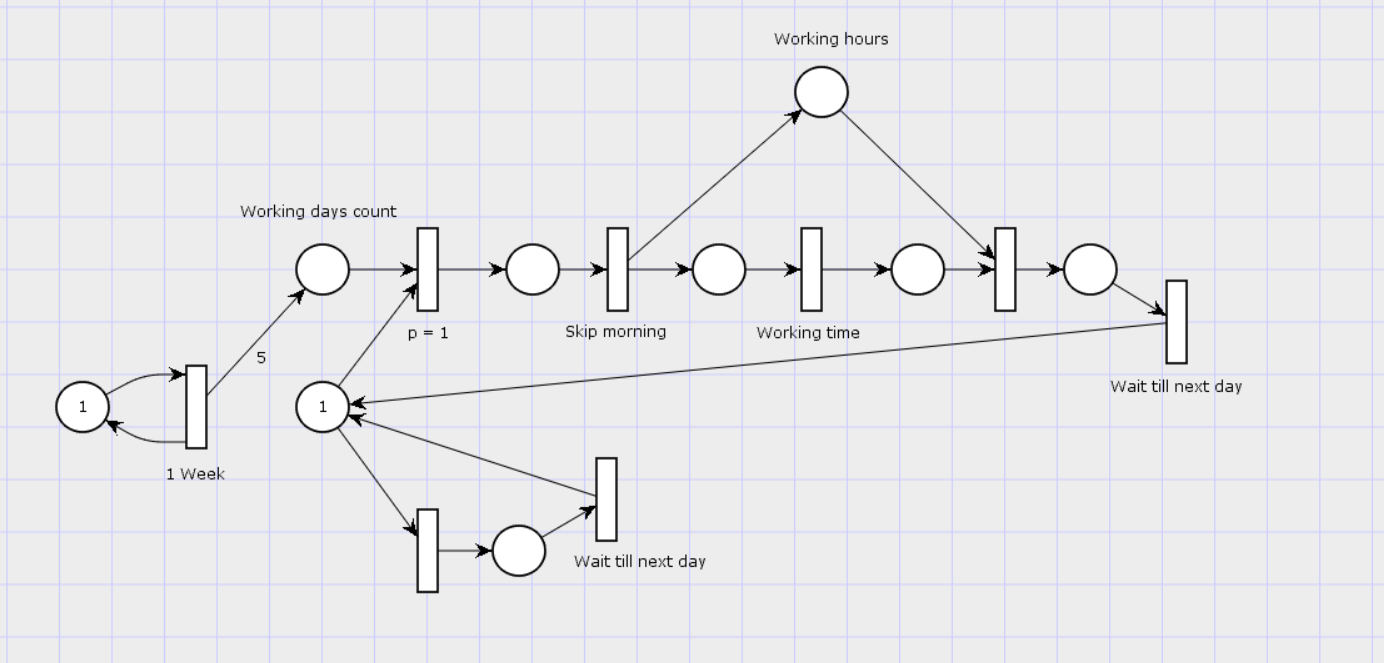
\includegraphics[scale=0.3]{img/WeekGen.png}
\caption{Transakce "Working hours" v době pracovní doby}
\end{figure}

\subsubsection{Simulace postřiku}
Modelujeme dva typy postřiku, ochranný a selektivní. Ochranný postřek se aplikuje na každý hektár pudy v daném období. Selektivní jenom na vybrané hektary pudy napadnuté škúdci.

\begin{figure}[ht!]
\centering
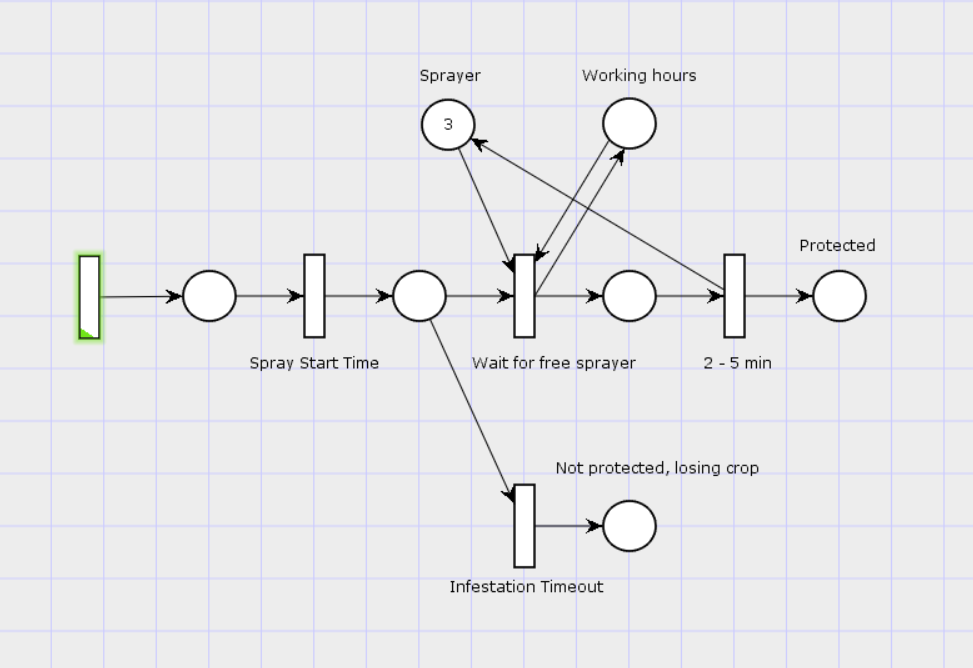
\includegraphics[scale=0.3]{img/SprayProt.png}
\caption{Průběh ochranného postřikování}
\end{figure}

\begin{figure}[ht!]
\centering
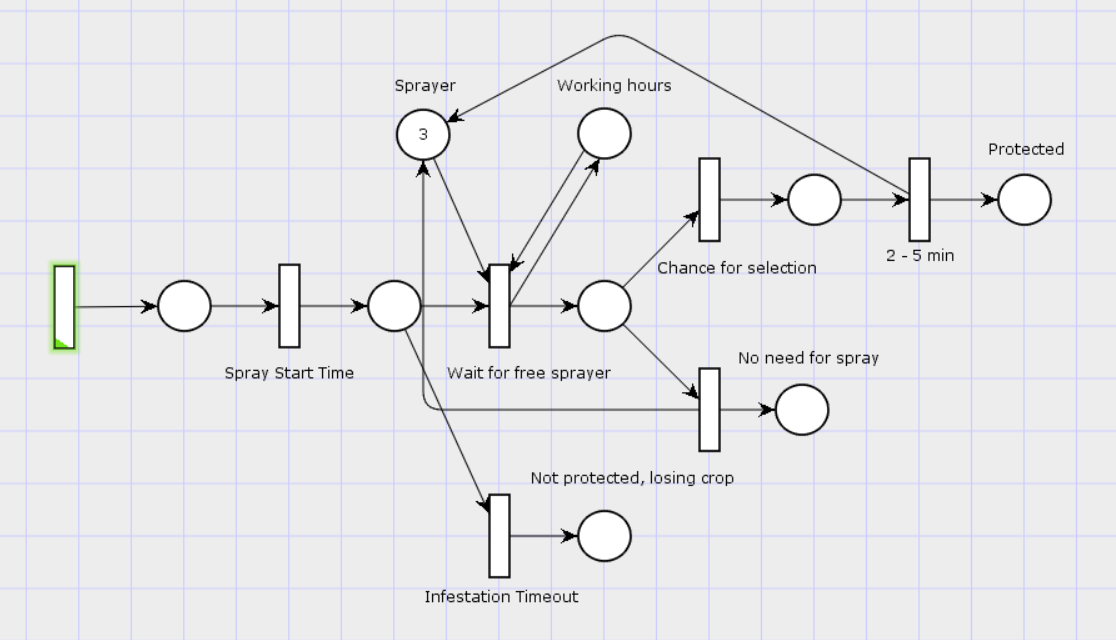
\includegraphics[scale=0.3]{img/SpraySel.png}
\caption{Průběh selektivního postřikování}
\end{figure}

\pagebreak

\subsubsection{Simulace hnojení}
Modelujeme dva typy hnojení. Jeden využíva ako obslužnú linku rozmetadlo minerálnych hnojiv a druhý poštrikové stroje. Rozmetadlo je využívané hnojivem Eurofertil Top 49 NPS. Ostatní hnojiva (Fertiactyl Starter, Fertileader Gold a Fertileader Vital) jsou nanášeny postřikem.

\begin{figure}[ht!]
\centering
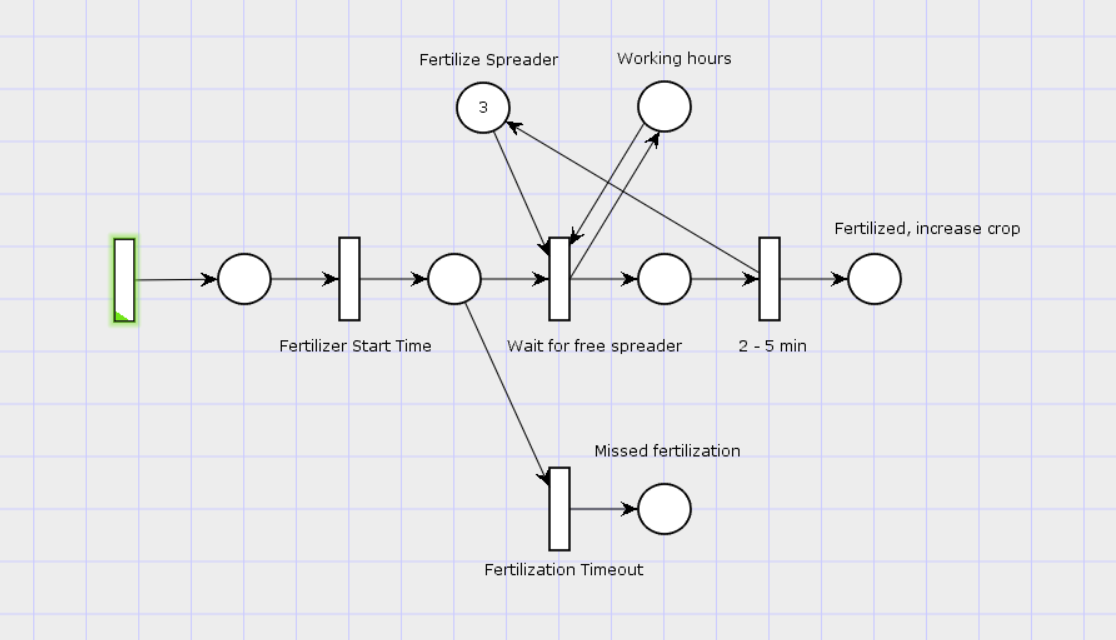
\includegraphics[scale=0.3]{img/FertilizationSpread.png}
\caption{Průběh hnojení za pomoci rozmetadla minerálnich hnojiv}
\end{figure}

\begin{figure}[ht!]
\centering
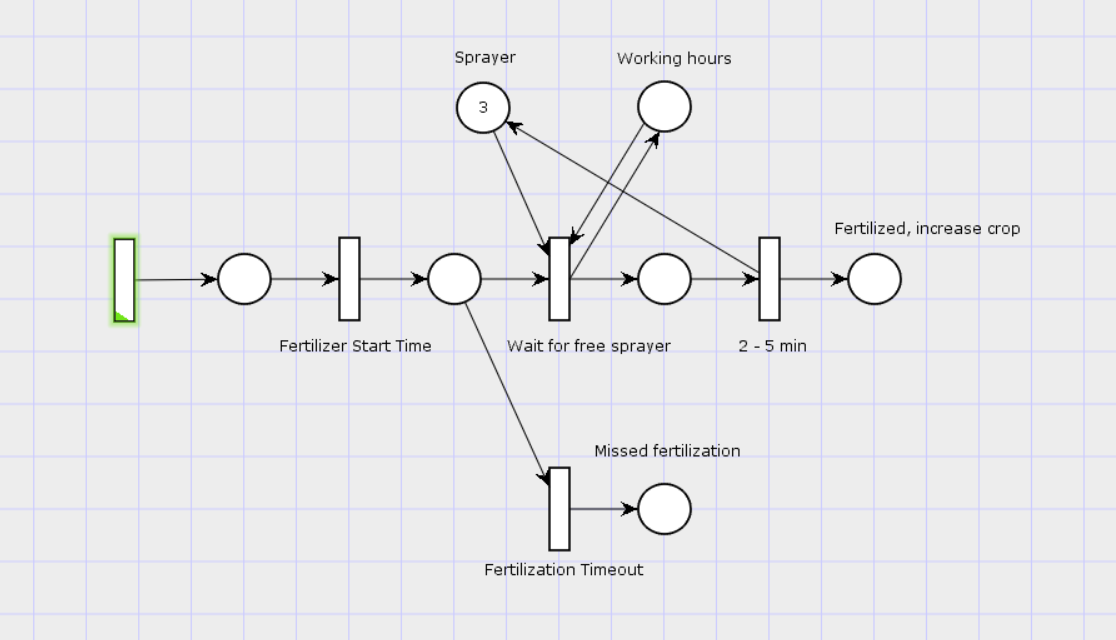
\includegraphics[scale=0.3]{img/FertilizationSpray.png}
\caption{Průběh hnojení za pomoci postřikového stroje}
\end{figure}

\pagebreak

\subsubsection{Simulace rustu}
Po úspešném zasetí každý hektar vygeneruje jednu transakci pro každý potřebný postřek či hnojení.

\begin{figure}[ht!]
\centering
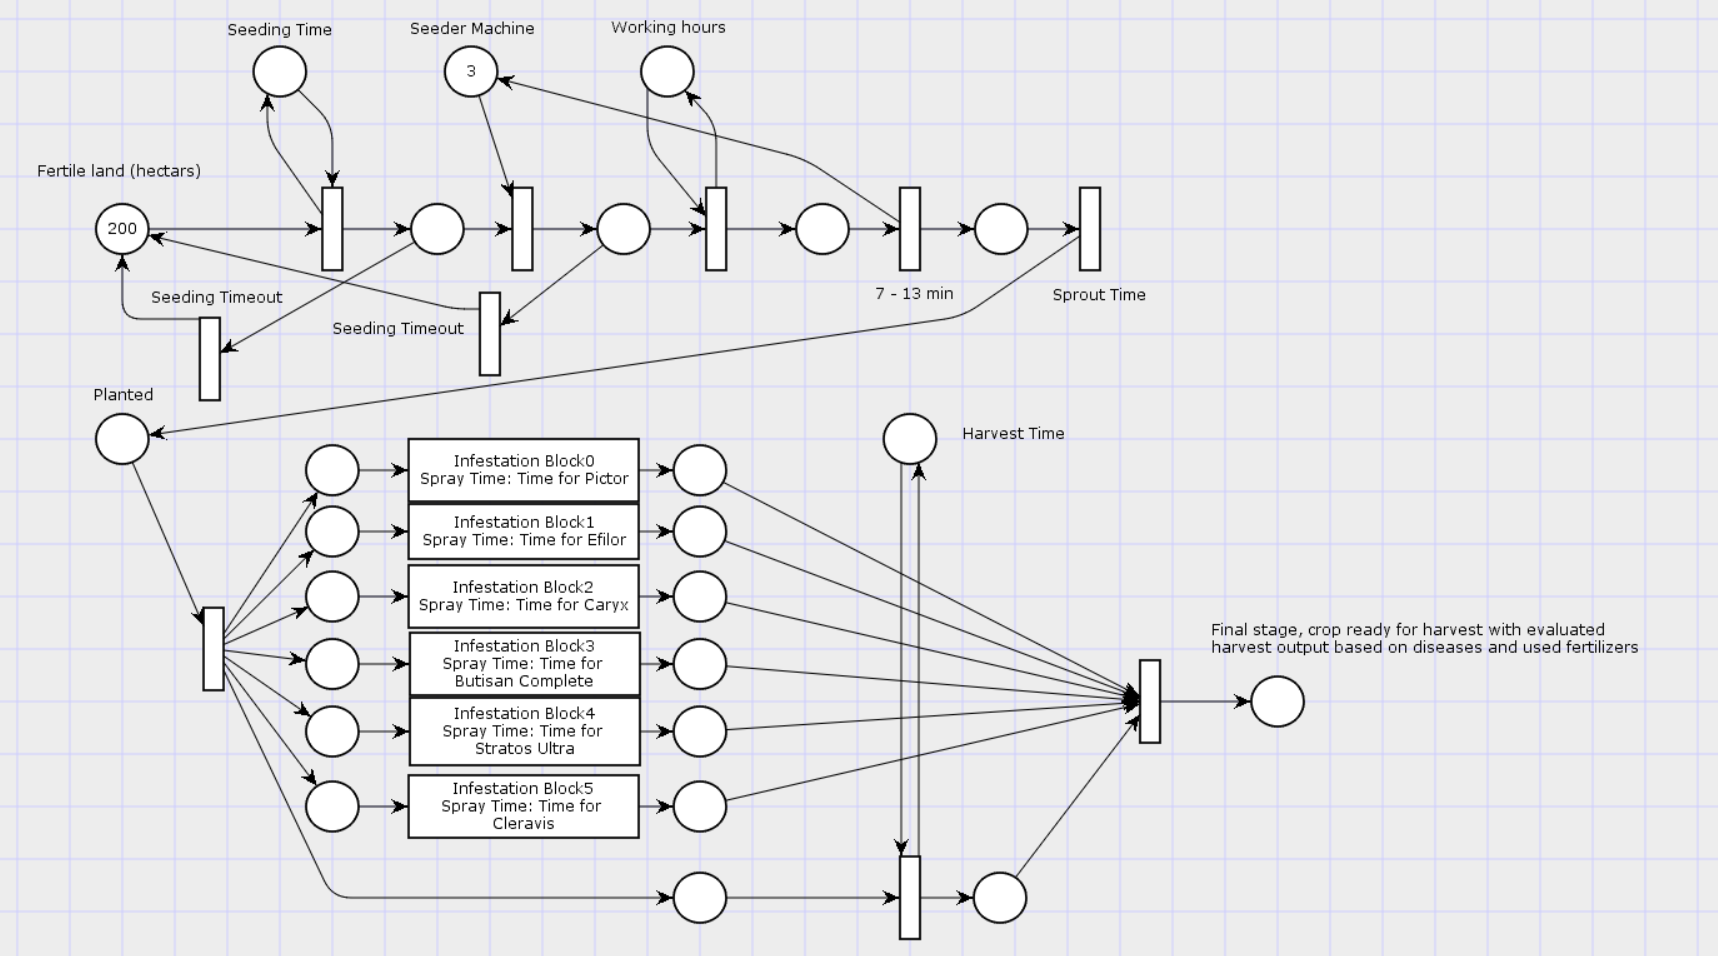
\includegraphics[scale=0.25]{img/Growing.png}
\caption{Růst řepky}
\end{figure}

\pagebreak

\subsubsection{Simulace sklizne}
Sklízecí mlátička sklidí pole a vrátí hektary spátky do místa \emph{Fertile Land}.

\begin{figure}[ht!]
\centering
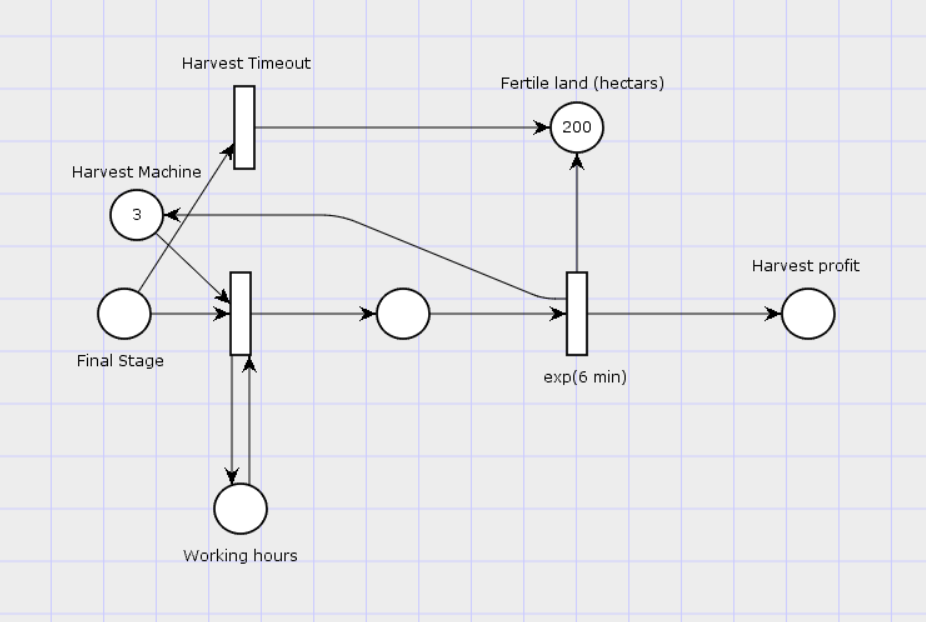
\includegraphics[scale=0.25]{img/Harvest.png}
\caption{Sklizeň}
\end{figure}

\pagebreak


\subsection{Parametry simulace}
Parametry simulace můžou být nastaveny v souboru \emph{"settings.conf"}. O jeho čtení se stará jednoduchý syntaktický analyzátor. Výrazy zapsané do tohoto souboru musí mít tvar: $$PARAMETR = hodnota$$ Výrazy musí být odděleny jedním nebo více prázdnými řádky. Cokoliv zapsané po sekvenci znakú \ceskeuvozovky{$//$} je bráno jako komentář, který bude syntaktickým analyzátorem ignorován.
\\ \\
Seznam Parametrů:
\begin{enumerate}
    \item{\emph{AVERAGEPROFIT} - představuje prumerný výnos v tunách řepky. potencionální zdroj téhle informace v české republice: https://www.vynosy-plodin.cz/2018-okresy-repka-ozima/, Výchozí hodnota je 2.5.}
    \item{\emph{WORKINGHOURSTIME} - představuje hodnotu v minutách v době, kdy se bude v pracovní dny pracovat. Výchozí hodnota je 480 (8 hodin).}
    \item{\emph{WORKINGDAYSCOUNT} - kolik pracovních dní má jeden týden. Výchozí hodnota je 5.}
    \item{\emph{MORNINGTIME} - představuje čas v minutách který se na začátku každého dne přeskočí, než se začne pracovat. Výchozí hodnota je 480 (8 hodin).}
    \item{\emph{TRACTORCOUNT} - kolik traktorů John Deere 6210R máme k dispozici. Výchozí hodnota je 3.}
    \item{\emph{SEEDINGMACHINECOUNT} - kolik secích strojů AMAZONE CAYENA máme k dispozici. Výchozí hodnota je 3.}
    \item{\emph{SPRAYERCOUNT} - kolik nesených postřikovačů AMAZONE UF máme k dispozici. Výchozí hodnota je 3.}
    \item{\emph{FERTILIZERSPREADERCOUNT} - kolik rozmetadel minerálních hnojiv AMAZONE ZA-M Ultra Profis Hydro máme k dispozici. Výchozí hodnota je 3.}
    \item{\emph{HARVESTMACHINECOUNT} - kolik sklízecích mlátiček New Holland CR10.90 máme k dispozici. Výchozí hodnota je 3.}
    \item{\emph{FERTILELANDCOUNT} - představuje počet hektárů půdy určených na růst řepky. Výchozí hodnota je 200.}
    \item{\emph{SEEDINGDURATION} - představuje čas v minutách vyhrazený na sázení řepky. Výchozí hodnota je 7200 (5 dnu).}
    \item{\emph{HARVESTDURATION} - představuje čas v minutách vyhrazený na sklizeň. Výchozí hodnota je 7200 (5 dnu).}
\end{enumerate}

\subsubsection{Zápis parametrú}
Parametry není nutno psát ve tvaru \ceskeuvozovky{\emph{WORKINGHOURSTIME}}, stejně dobře funguje i zápis \ceskeuvozovky{\emph{Working Hours Time}}, \ceskeuvozovky{\emph{working hours time}} nebo \ceskeuvozovky{\emph{workingHours Time}}. Při zápisu parametru nezávisí na velikosti písmen ani na mezerách. Když bude hodnota za \ceskeuvozovky{$=$} neplatná, nebo když nebude některý z parametrů uveden v konfiguračním souboru, použije se jeho výchozí hodnota.

\section{Příklad použití}

Představme si následující situaci: \\
Vlastníme pole o rozloze 500 hektarů, máme 3 secí stroje, 3 traktory a 1 rozmetadlo minerálních hnojiv. Zajíma nás kolik postřikovacích strojů budeme potřebovat. \\ \\

Proto jako první nastavíme dané parametry do konfiguračního souboru asi nějak takto: \\

\begin{lstlisting}
//Example 1

Fertile Land Count = 500    //area in hectars

Average Profit = 2.0

Working Hours Time = 480 //duration of daily shift in minutes
Working Days Count = 5
Morning Time = 480 //duration in minutes which will be skiped every day before shift start

Seeding Machine Count = 3
Tractor Count = 3
Sprayer Count = 1
Fertilizer Spreader Count = 1
Harvest Machine Count = 2

SEEDINGDURATION = 7200 //duration of seeding in minutes
HARVESTDURATION = 7200 //duration of harvest in minutes
\end{lstlisting}


\newpage
\bibliography{literatura}

\end{document}
